\documentclass[10pt,a4paper]{article}
\usepackage[T1]{fontenc}
\usepackage[utf8]{inputenc}
\usepackage{lmodern,graphicx,booktabs,geometry,hyperref}
\geometry{margin=22mm}
\setlength{\parindent}{0pt}
\setlength{\parskip}{5pt}
\pagestyle{plain}
\begin{document}
{\LARGE\bfseries Lancer plus tôt, regrouper davantage\par}
{\large Livraison à l'heure sur une ligne S-DBR à dix postes\par}
\section*{Comparer à plafond de lot constant}
À quelle fenêtre de lancement les commandes ont-elles le plus de chances d'être
expédiées avant leur échéance ? Le graphique compare cinq minima fixes et deux
minima croissants. Tous autorisent des lots de seize au maximum, y compris
la référence fixe1. Chaque marque correspond à dix réplications.
\begin{center}
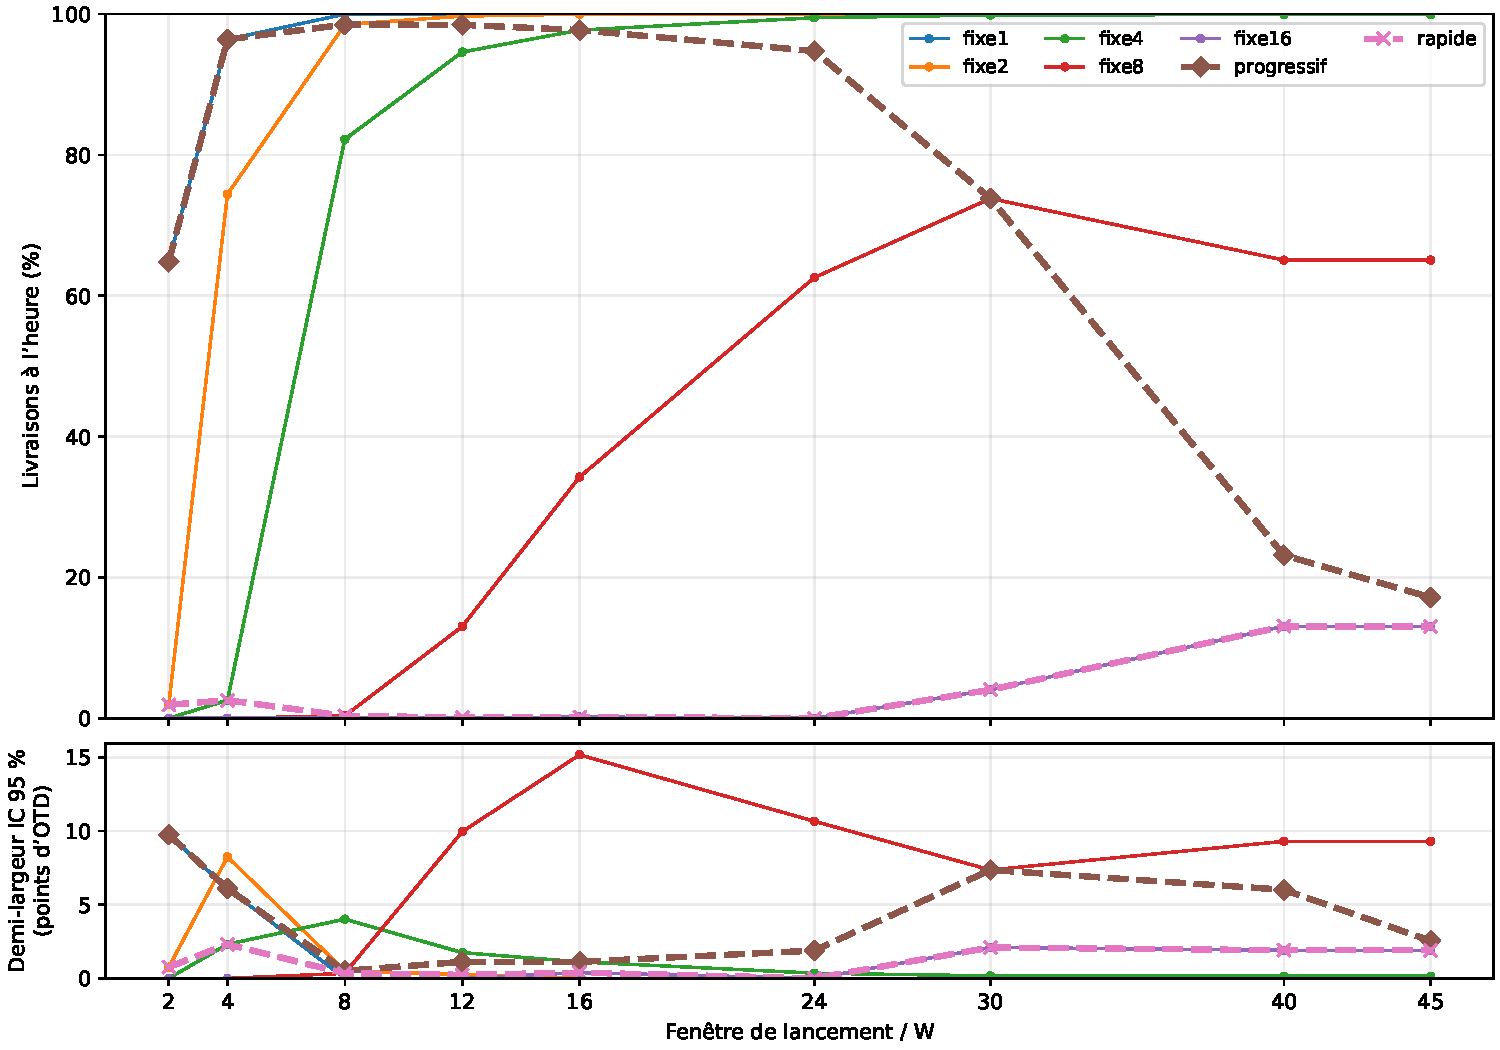
\includegraphics[width=\linewidth,height=.45\textheight,keepaspectratio]{otd-fenetre.pdf}

\small\begin{tabular}{lrrrrrrrrr}\toprule
Fenêtre / W & 2 & 4 & 8 & 12 & 16 & 24 & 30 & 40 & 45 \\
progressif & 1 & 1 & 2 & 3 & 4 & 6 & 8 & 10 & 11 \\
rapide & 2 & 4 & 8 & 12 & 16 & 16 & 16 & 16 & 16 \\

\end{tabular}

Minimum demandé pour chaque point des deux courbes en tirets.
\end{center}
Suivre une ligne fine isole l'effet de la fenêtre pour un minimum donné.
Suivre une ligne en tirets combine anticipation et regroupement. Une lecture
verticale compare deux minima pour la même fenêtre. Les courbes se superposent
lorsque les paramètres effectifs coïncident. Le panneau inférieur donne la
demi-largeur de chaque intervalle de confiance (IC), en points de pourcentage.
\newpage
\section*{Ce que propose Goldratt}
Dans \emph{Standing on the shoulders of Giants}, Goldratt décrit comment la place
disponible chez Ford et les signaux de réapprovisionnement chez Toyota limitent
le travail lancé. La recherche d'occupation maximale à chaque poste peut aller
à l'encontre du flux de la ligne (pp.~3--7). Les conditions de stabilité du
système Toyota comptent lorsqu'on transpose ces pratiques (pp.~8--10).

Pour une production sur commande, Goldratt examine le lancement en fonction du
temps restant avant la date promise. Si cette marge couvre à peine le travail
opératoire, une file ou un aléa suffit à la consommer. Une marge plus généreuse
absorbe ces aléas. Mais lancer très tôt multiplie les ordres présents, les files
et les arbitrages de priorité. L'ordonnée de sa figure~1 est \emph{l'attention
managériale nécessaire pour tenir les délais} (pp.~12--14). Ici, la politique
d'ordonnancement est automatique et l'on mesure le pourcentage de commandes
livrées à l'heure. Le lien entre les deux grandeurs est une hypothèse à examiner.

Goldratt invite aussi à compter le temps qu'une pièce attend pendant qu'une
autre est travaillée dans le même lot (p.~13). Nous introduisons une règle
expérimentale spécifique : demander des lots plus grands lorsque la fenêtre
s'allonge. Cette règle permet de rechercher un mécanisme susceptible de dégrader
le service malgré une mise en production plus précoce.

\section*{Protocole apparié}
Le contenu de travail nominal moyen $W$ vaut environ 54,3 h. Pour une commande
reçue en $a$ et promise en $d$, la libération a lieu en $\max(a,d-xW)$.
Les délais demandés suivent une loi uniforme de $10W$ à $40W$. À $40W$ et
$45W$, toute commande est donc libérée dès sa réception. Pour les politiques
variables, le minimum demandé vaut
$\min(16,\max(1,\mathrm{arrondi}(kx)))$, avec $k=0{,}25$ (progressif) ou
$k=1$ (rapide). L'arrondi porte sur les heures effectivement simulées.

La ligne comprend quatre familles, un goulot au cinquième poste, des tampons de
16 et des transferts unitaires. Chaque poste privilégie sa famille courante si
elle est admissible, puis la première famille admissible dans l'ordre d'arrivée.
Après 168 h d'attente de sa plus ancienne pièce, une famille peut partir sous le
minimum. La taille observée peut ainsi différer du minimum demandé.

Les graines 42 à 51 reproduisent, pour chaque politique et fenêtre, les mêmes
arrivées, familles, dates promises et durées opératoires. Le CV des interarrivées
vaut 1 à charge constante et celui des durées opératoires lognormales vaut 0,60.
Après 400 h de chauffe, les charges successives sont de 70, 95, 130 et 85\,\%
pendant 480, 720, 480 et 720 h. L'OTD porte sur les commandes dues entre 400 h
(incluses) et 2\,800 h (exclues). Le simulateur poursuit les arrivées jusqu'à la
fin de l'observation augmentée du délai client maximal et vide la ligne jusqu'à
la dernière expédition. Une commande de la cohorte livrée après l'horizon reste
comptée dans l'OTD.
\newpage
\section*{Fenêtres donnant le meilleur service observé}
\small
\begin{tabular}{l l r l}\toprule
Politique & Fenêtre ($W$) & OTD (\%) & Voisin : gain en points [IC 95\,\%]\\\midrule
fixe1 & 8, 12, 16, 24, 30, 40, 45 & 100.0 & 4 W : 3.6 [-2.5, 9.7] / 12 W : 0.0 [0.0, 0.0] \\
fixe16 & 40, 45 & 13.1 & 30 W : 9.0 [5.9, 12.1] / 45 W : 0.0 [0.0, 0.0] \\
fixe2 & 16, 24, 30, 40, 45 & 100.0 & 12 W : 0.3 [0.0, 0.5] / 24 W : 0.0 [0.0, 0.0] \\
fixe4 & 40, 45 & 99.9 & 30 W : 0.0 [-0.2, 0.3] / 45 W : 0.0 [0.0, 0.0] \\
fixe8 & 30 & 73.8 & 24 W : 11.2 [2.9, 19.6] / 40 W : 8.8 [-0.5, 18.0] \\
progressif & 8 & 98.5 & 4 W : 2.1 [-3.6, 7.8] / 12 W : 0.0 [-1.2, 1.3] \\
rapide & 40, 45 & 13.1 & 30 W : 9.0 [5.9, 12.1] / 45 W : 0.0 [0.0, 0.0] \\

\end{tabular}
\normalsize

Les fenêtres ex æquo sont indiquées ensemble. Le gain est calculé graine par
graine entre le premier maximum et chacune des fenêtres adjacentes. Un intervalle
contenant zéro laisse le sens de l'écart incertain. Les IC utilisent la loi de
Student à neuf degrés de liberté ; ils décrivent ces dix réplications, sans
correction pour la sélection du meilleur point ou les comparaisons multiples.

\section*{Que se passe-t-il dans l'atelier ?}
\small
\begin{tabular}{lrrrrrrrr}\toprule
Politique & $x$ & Min. & OTD \% & En cours & Cycle h & CV cycle & Lot réel & Attente h\\\midrule
fixe1 & 2 & 1 & 64.8 & 8.2 & 107 & 0.33 & 1.4 & 0 \\
fixe1 & 8 & 1 & 100.0 & 11.1 & 107 & 0.33 & 1.5 & 0 \\
fixe1 & 45 & 1 & 100.0 & 21.7 & 127 & 0.42 & 1.9 & 0 \\
progressif & 2 & 1 & 64.8 & 8.2 & 107 & 0.33 & 1.4 & 0 \\
progressif & 8 & 2 & 98.5 & 18.3 & 193 & 0.37 & 2.8 & 238 \\
progressif & 45 & 11 & 17.2 & 169.8 & 1663 & 0.12 & 11.8 & 270 \\
rapide & 2 & 2 & 1.9 & 14.3 & 193 & 0.37 & 2.8 & 223 \\
rapide & 8 & 8 & 0.3 & 68.4 & 957 & 0.30 & 8.1 & 801 \\
rapide & 45 & 16 & 13.1 & 175.0 & 1780 & 0.11 & 11.6 & 323 \\

\end{tabular}
\normalsize

L'en-cours compte les ordres présents en moyenne temporelle. Le cycle va de la
libération à l'expédition. Le lot réel est la taille moyenne de série mesurée
sur les postes. L'attente mesure les heures où le goulot, libre et non bloqué,
a des pièces en file mais aucun lot admissible. Elle exclut le temps pendant
lequel il sert une autre famille. Ces grandeurs sont moyennées sur les graines.

\section*{Décider de la fenêtre et du minimum}
À minimum fixe de 1, élargir la fenêtre de $2W$ à $8W$ relève l'OTD de
35,2 points alors que la traversée moyenne reste proche de 107 h. La marge
avant échéance aide donc à absorber les aléas. À $45W$, l'en-cours a presque
doublé par rapport à $8W$ et l'OTD reste à 100\,\% sur ces graines. Une hausse
de l'en-cours seule ne suffit pas ici à dégrader le service.

Le couplage progressif donne 98,5\,\% à $8W$ et 17,2\,\% à $45W$.
L'écart en faveur du minimum fixe de 1, à fenêtre identique, passe de
1,5 point [1,0 ; 2,0] à 82,8 points [80,3 ; 85,4]. Les séries effectivement
formées grossissent, la traversée moyenne dépasse 1\,660 h et le goulot attend
des regroupements pendant 270 h à $45W$. Cette dernière mesure ne représente
qu'une partie de l'attente dans une ligne à dix postes ; elle ne permet pas
d'attribuer à elle seule toute la perte d'OTD.

Pour cette usine et cet objectif de service, un minimum de 1 et une fenêtre
de $8W$ atteignent déjà le plateau observé avec environ onze ordres en cours.
Si le lot doit croître avec la fenêtre, les données favorisent le couplage
progressif autour de $8W$ à $12W$ ; dix graines ne départagent pas ces deux
fenêtres. Le couplage rapide reste sous 14\,\% même à son meilleur point.
La branche descendante de l'OTD dépend donc de la politique adoptée. Cette
expérience quantifie un mécanisme compatible avec le raisonnement de Goldratt,
sans mesurer directement les interventions humaines.


\small\textit{Source primaire.} E. M. Goldratt, \emph{Standing on the shoulders
of Giants: Production concepts versus production applications. The Hitachi Tool
Engineering Example}, édition du dépôt, figure 1 et pages indiquées ci-dessus.
\end{document}
